\section{Simulación} \label{sec:simulacion}

Siguiendo el tutorial comenzamos ensamblando nuestro robot, y marcando sus ejes dentro del programa de SolidWorks.

\begin{figure}[h]
	\centering
	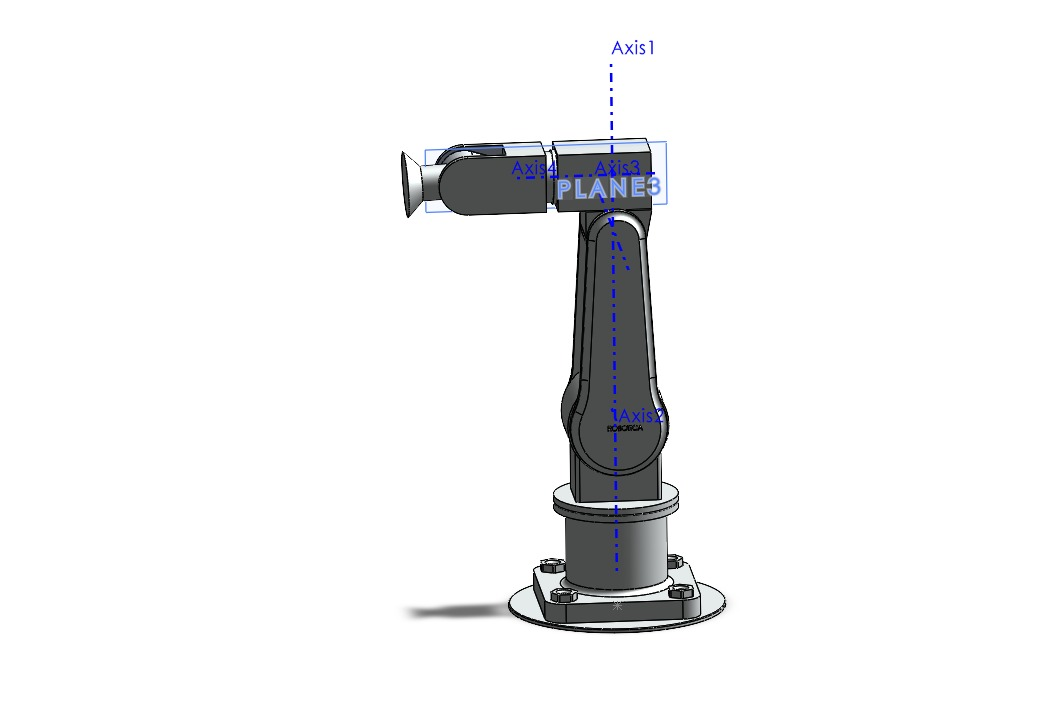
\includegraphics[width=0.75\textwidth]{img/ROBOT SOLID}
	\caption{Robot ensamblado en SolidWorks}
	\label{fig:ROBOT SOLID}
\end{figure}

Posteriormente se colocan los límites de giro del brazo, así como el torque y velocidad.


\begin{figure}[H]
	\centering
	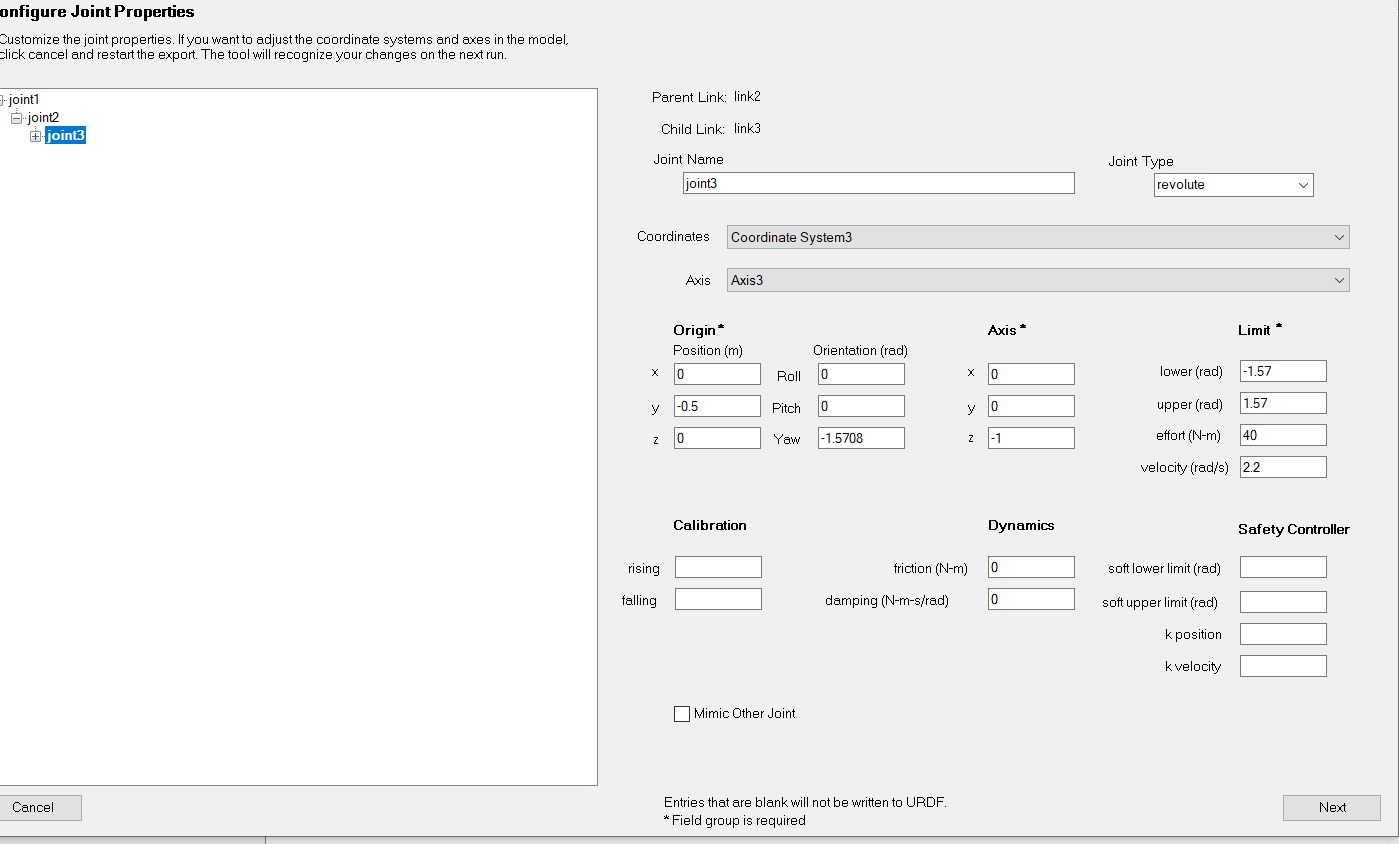
\includegraphics[width=0.75\textwidth]{img/limitessolidrobot}
	\caption{Limites del robot en SolidWorks}
	\label{fig:Limites del robot en SolidWorks}
\end{figure}
  
  
\newpage

Después utilizamos el simulador https://gkjohnson.github.io/urdf-loaders/javascript/example/bundle/   para comprobar que el movimiento del robot sea el esperado.

\begin{figure}[H]
	\centering
	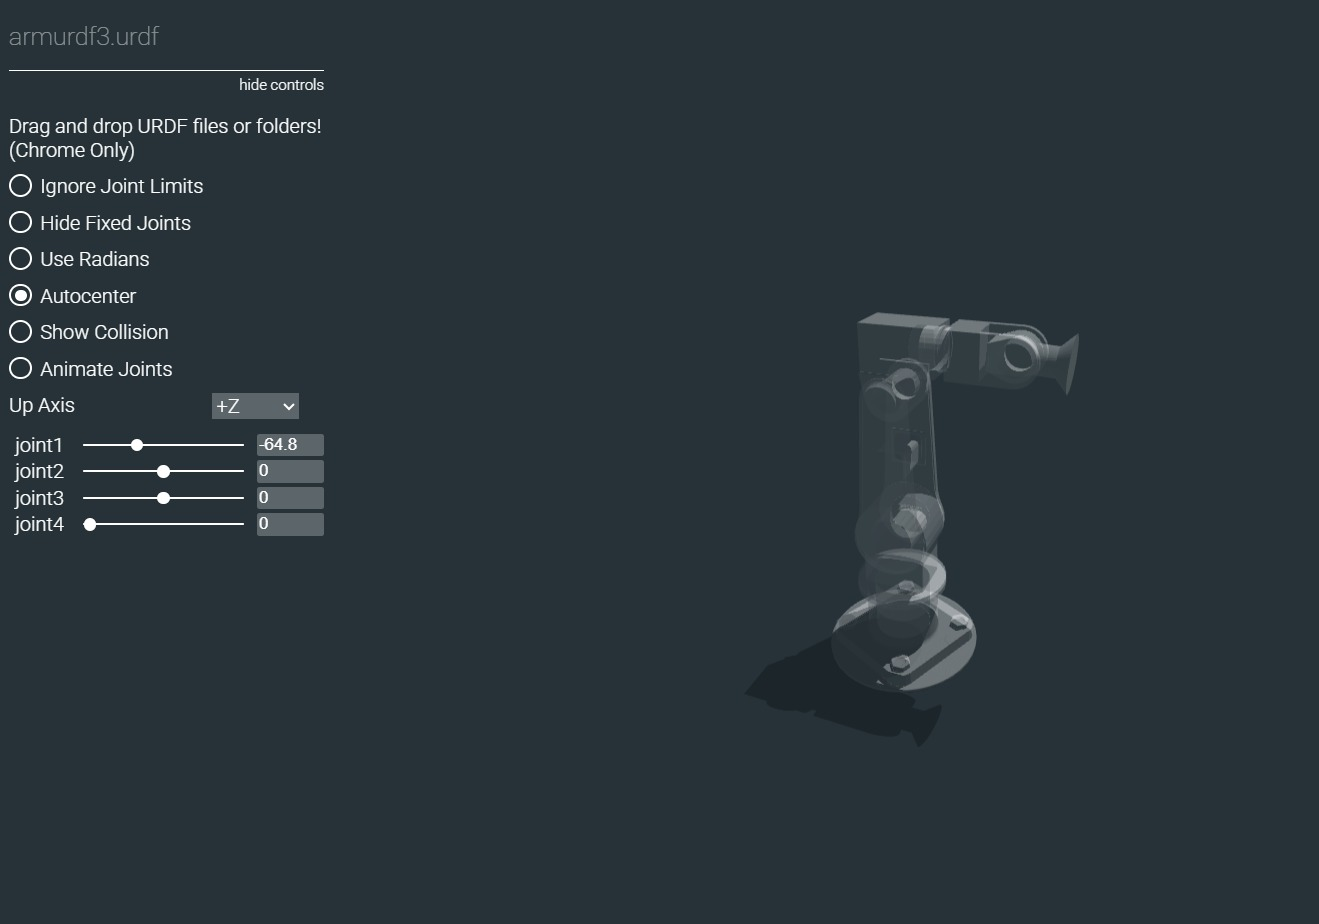
\includegraphics[width=0.75\textwidth]{img/robotsimulado}
	\caption{Robot simulado}
	\label{fig:Robot simulado}
\end{figure}

Se siguieron los pasos establecidos en el tutorial del profesor 
\href{https://www.youtube.com/watch?v=p9g-5OLhynA&list=PLeEzO_sX5H6TBD6EMGgV-qdhzxPY19m12&index=1&ab_channel=AgeofRobotics}{(ver tutorial en YouTube)} 
para poder usar nuestro archivo URDF en ROS.

Usando ubuntu 20.04 mediante WSL, desde Visual Studio, se siguieron todos los pasos establecidos, modificando los archivos requeridos para adaptarlos a nuestro robot (ejemplo: se eliminó todos lo relacionado a pinzas, así como se delimitaron los joints a una cantidad de 4, debido a que es la cantidad de articulaciones de nuestro robot) y así poder simular correctamente. Dicha simulación se realizó de manera exitosa, y se puede ver en la sección de resultados.

